\documentclass[
    % fontset=ubuntu, % 生僻字可用思源字体,如“昇腾”
    fontset=fandol,
    xcolor=svgnames % SeaGreen
]{ctexbeamer}

\usepackage{pgfplots}

\usetheme[
    compress % 进度条压缩在一行,可选
]{Berlin}

\usecolortheme[named=SeaGreen]{structure}

\title[面向国产异构处理器的HPL-AI基准实现及优化]{面向国产异构处理器的HPL-AI基准实现优化}

\subtitle[申请中山大学工学学士学位论文答辩报告]{
    ~\\
    (申请中山大学工学学士学位论文答辩报告)
}

\author[吴坎]{
    \texorpdfstring{
        学生:吴坎\\
        ~\\
        \href{mailto:wukan3@mail2.sysu.edu.cn}{wukan3@mail2.sysu.edu.cn}
    }{PDF Bookmark Version}
}

\institute[中山大学~计算机学院(软件学院)~计算机科学与技术(超算方向)]{
    \includegraphics[height=0.1\textheight]{../image/template/logo.png}
    % \includegraphics[height=0.1\textheight]{../image/template/sysu-logo.pdf} % 这里可以放一排所在实验室的logo,可以去学院官网底部或实验室主页弄到,如 <http://nscc-gz.cn/_layout/themes/cs/images/logo0409.png>
}

\logo{\includegraphics[height=0.1\textheight]{../image/template/sysu-logo.pdf}} % 这个是每页都会出现的水印,可能会影响观感,自行决定放不放

\date{
    %\today
    二〇二一年五月
}

\begin{document}

\section{Intro}

\begin{frame}

    \titlepage

\end{frame}

\subsection{选题背景}

\begin{frame}
    \begin{block}{Linpack\footnote{\url{http://www.netlib.org/linpack/}}是国际上最受认可的高性能计算机基准}
        \begin{itemize}
            \item 是TOP500超算排名的唯一参照
        \end{itemize}
    \end{block}
    \begin{block}{现代超算越来越多地被用于人工智能应用}
        \begin{itemize}
            \item 模型使用包括单精度、半精度在内的混合精度加速
        \end{itemize}
    \end{block}
    \begin{block}{各种新型计算设备不断推出}
        \begin{itemize}
            \item GPU、TPU、NPU、FPGA……
        \end{itemize}
    \end{block}
    \begin{block}{Linpack基准存在局限性}
        \begin{itemize}
            \item 仅能衡量计算系统双精度求解能力
        \end{itemize}
    \end{block}
\end{frame}

\subsection{国内外研究现状}

\begin{frame}
    \begin{itemize}
        \item 2019年,J. Dongarra 对 Linpack 基准进行扩展
              \begin{itemize}
                  \item 新基准被称作 HPL-AI\footnote{\url{https://icl.bitbucket.io/hpl-ai/}}
                  \item 在矩阵求解过程中放弃双精度计算的要求
                  \item 使用数值迭代手段,恢复在低精度运算中损失的精度
                  \item 可利用已有的或即将推出的 AI 设备来加速求解过程
              \end{itemize}
        \item Summit\footnote{\url{https://www.top500.org/system/179397/}}在HPL-AI中得到了三倍于Linpack的效率
        \item Fugaku\footnote{\url{https://www.top500.org/system/179807/}}首次将求解速度提升至Eflops量级
    \end{itemize}
\end{frame}

\subsection{本文解决的问题}

\begin{frame}
    \begin{block}{尚未有可用于大规模测试的HPL-AI开源实现}\begin{itemize}
            \item 目前的开源实现仅有J. Dongarra提供的单线程参考版本\footnote{\url{https://bitbucket.org/icl/hpl-ai/}}
        \end{itemize}
    \end{block}
    \begin{block}{尚未有CPU、GPU等通用平台之外的HPL-AI评测}\begin{itemize}
            \item 如何对国产异构处理器(NPU)实现大规模性能评测?
        \end{itemize}
    \end{block}
\end{frame}

\section{HPL-AI算法分析}
\begin{frame}
    \begin{block}{HPL-AI主要思想}
        \begin{itemize}
            \item 对矩阵混合精度分解,计算较低精度下得到的近似解
            \item 使用双精度的数值迭代,得到与双精度分解相当的精确度
        \end{itemize}
    \end{block}
    \begin{block}{使用算法}
        \begin{itemize}
            \item 矩阵构造算法
            \item 并行LU分解算法(PGESV)
            \item 并行广义最小残差算法(PGMRES)
        \end{itemize}
    \end{block}
\end{frame}
\subsection{面临的挑战}
\begin{frame}
    \begin{block}{针对硬件的算法设计}
        \begin{itemize}
            \item 基于全新的国产异构芯片设计算法
            \item 混合精度策略选择
        \end{itemize}
    \end{block}
    \begin{block}{异构计算中的负载均衡问题}
        \begin{itemize}
            \item Device与Host协同计算
            \item 高性能BLAS/MPI调用实现
        \end{itemize}
    \end{block}
\end{frame}

\section{实现与移植工作}
\subsection{Ascend910硬件架构}
\begin{frame}
    \begin{itemize}
        \item 矩阵计算单元 Cube Unit
        \item 向量计算单元 Vector Unit
        \item 标量计算单元 Scalar Unit
    \end{itemize}
    \begin{figure}[h]
        \centering
        \includegraphics[width=0.8\textwidth]{../image/chap03/davinci.png}
        \caption{达芬奇架构图}
        \label{达芬奇架构图}
    \end{figure}
\end{frame}

\subsection{基于Profile实验的结论}
\begin{frame}
    \begin{block}{上下文创建/释放、设备内存申请/释放的开销都很大}
        \begin{itemize}
            \item 需要在运行算法时尽量避免无关调用
        \end{itemize}
    \end{block}
    \begin{block}{MatMul 算子调用时间远低于 aclrtMemcpy(5ms:35ms)}
        \begin{itemize}
            \item 需要将部分计算量移动到Host端,掩盖通信
        \end{itemize}
    \end{block}
    \begin{block}{GEMM 算子性能远低于 MatMul 和 MatMulV2}
        \begin{itemize}
            \item 合理推断:向量/标量单元性能远低于矩阵单元
        \end{itemize}
    \end{block}
\end{frame}

\subsection{移植方案}
\begin{frame}
    \begin{itemize}
        \item 将GEMM($C\leftarrow \alpha AB+\beta C$)调用进一步拆分
              \begin{itemize}
                  \item 在Device端调用MatMul算子
                  \item 在Host端做系数乘
              \end{itemize}
        \item 针对硬件的混合精度算法
              \begin{itemize}
                  \item MatMul:FP16
                  \item PGESV:FP32
                  \item PGMRES:FP64
              \end{itemize}
        \item 基于矩阵分块的负载均衡算法
        \item 懒释放+热身运行策略
              \begin{itemize}
                  \item 减少无关调用
              \end{itemize}
    \end{itemize}
\end{frame}

\begin{frame}
    \begin{itemize}
        \item 优化的矩阵布局
              \begin{itemize}
                  \item 减少Device端内存占用
              \end{itemize}
    \end{itemize}

    \begin{figure}[h]
        \centering
        \begin{tabular}{cccccc}
            \cline{1-5}
            \multicolumn{1}{|c|}{}           & \multicolumn{1}{c|}{hB} & \multicolumn{1}{c|}{hA} & \multicolumn{1}{c|}{sA} & \multicolumn{1}{c|}{sB} & Copy+Cast阶段 \\ \cline{1-5}
            \multicolumn{5}{c}{$\downarrow$} &                                                                                                                       \\ \cline{1-5}
            \multicolumn{1}{|c|}{hC}         & \multicolumn{1}{c|}{hB} & \multicolumn{1}{c|}{hA} & \multicolumn{2}{c|}{}   & MatMul阶段                              \\ \cline{1-5}
            \multicolumn{5}{c}{$\downarrow$} &                                                                                                                       \\ \cline{1-5}
            \multicolumn{1}{|c|}{hC}         & \multicolumn{4}{c|}{sC} & Cast+Copy阶段                                                                               \\ \cline{1-5}
        \end{tabular}
        \caption{内存排布图示}
        \label{内存排布图示}
    \end{figure}
\end{frame}

\section{实验与分析}
\subsection{可扩展性验证实验}

\begin{frame}
    \begin{itemize}
        \item 问题规模足够大时,固定问题规模N,求解效率随并行核数增加线性增长
        \item 我们的实现有强可扩展性
    \end{itemize}

    \pgfplotsset{width=0.6\textwidth}
    \begin{figure}
        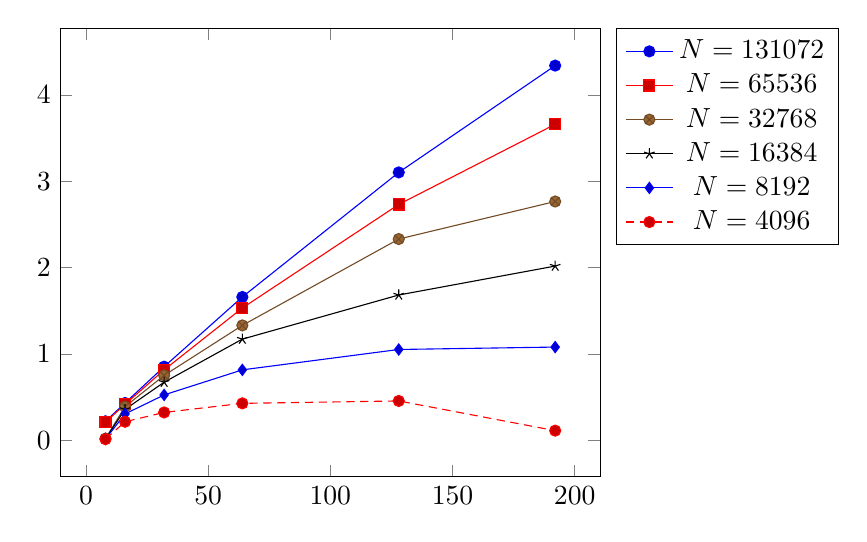
\begin{tikzpicture}
            \begin{axis}[legend pos=outer north east] % 将图例放在图外,位于图的东北角
                \addplot
                coordinates                             % 绘制原始数据的折线图
                    {           		                % X,Y的原始数据
                        (8,0.22)
                        (16,0.432)
                        (32,0.853)
                        (64,1.660)
                        (128,3.103)
                        (192,4.340)
                    };
                \addlegendentry{$N=131072$}
                \addplot
                coordinates                              % 绘制原始数据的折线图
                    {           		                % X,Y的原始数据
                        (8,0.21)
                        (16,0.417)
                        (32,0.816)
                        (64,1.532)
                        (128,2.732)
                        (192,3.660)
                    };
                \addlegendentry{$N=65536$}
                \addplot
                coordinates                                 % 绘制原始数据的折线图
                    {           		                % X,Y的原始数据
                        (8,0.020)
                        (16,0.389)
                        (32,0.752)
                        (64,1.331)
                        (128,2.331)
                        (192,2.766)
                    };
                \addlegendentry{$N=32768$}
                \addplot
                coordinates                                 % 绘制原始数据的折线图
                    {           		                % X,Y的原始数据
                        (8,0.019)
                        (16,0.358)
                        (32,0.673)
                        (64,1.172)
                        (128,1.683)
                        (192,2.018)
                    };
                \addlegendentry{$N=16384$}
                \addplot
                coordinates                                 % 绘制原始数据的折线图
                    {           		                % X,Y的原始数据
                        (8,0.016)
                        (16,0.305)
                        (32,0.526)
                        (64,0.816)
                        (128,1.052)
                        (192,1.080)
                    };
                \addlegendentry{$N=8192$}
                \addplot
                coordinates                               % 绘制原始数据的折线图
                    {           		                % X,Y的原始数据
                        (8,0.013)
                        (16,0.215)
                        (32,0.323)
                        (64,0.428)
                        (128,0.456)
                        (192,0.112)
                    };
                \addlegendentry{$N=4096$}
            \end{axis}
        \end{tikzpicture}
        \caption{HPL-AI具有强可扩展性}
        \label{HPL-AI具有强可扩展性}
    \end{figure}

\end{frame}

\subsection{NPU加速验证实验}

\begin{frame}
    \begin{itemize}
        \item 相对于HPL,HPL-AI取得2.59x加速比
        \item HPL-AI可通过异构处理器获得明显性能提升
        \item 引入半精度的计算可以获得更高求解效率
    \end{itemize}

    \pgfplotsset{width=0.6\textwidth}
    \begin{figure}
        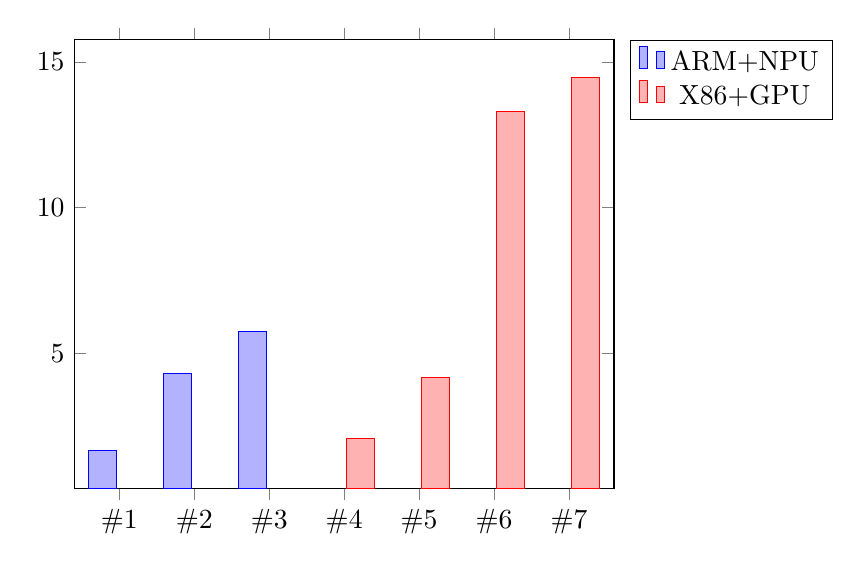
\begin{tikzpicture}
            \begin{axis}
                [
                    ybar,
                    symbolic x coords={\#1, \#2, \#3, \#4, \#5, \#6, \#7},
                    legend pos=outer north east
                ]

                \addplot coordinates {(\#1, 1.657) (\#2, 4.296) (\#3, 5.733)};
                \addlegendentry{ARM+NPU};
                \addplot coordinates {(\#4, 2.088) (\#5, 4.162) (\#6, 13.291) (\#7, 14.477)};
                \addlegendentry{X86+GPU};

            \end{axis}
        \end{tikzpicture}
        \caption{实测性能对照图}
        \label{实测性能对照图}
    \end{figure}

\end{frame}

\begin{frame}

    \begin{block}{NPU运行HPL-AI的瓶颈在于Host-Device通信}
        \begin{itemize}
            \item PCIe4.0带宽相较NVLink低十倍
            \item 若后续Ascend处理器提升与主机的带宽,可在HPL-AI基准中获得更高的计算效率
        \end{itemize}
    \end{block}
    \begin{block}{NVIDIA GPU可以使用优化的cuBLAS计算库}
        \begin{itemize}
            \item Ascend平台在软件生态建设上任重而道远
        \end{itemize}
    \end{block}

\end{frame}

\section{总结与展望}
\subsection{总结}
\begin{frame}
    \begin{block}{本文工作}
        \begin{itemize}
            \item 首个开源的分布式HPL-AI基准实现
            \item 针对国产异构处理器——Ascend 910进行移植与优化
            \item 在X86、ARM、GPU、NPU等多个平台上运行基准
        \end{itemize}
    \end{block}
    \begin{block}{意义}
        \begin{itemize}
            \item 为不同平台上的HPL-AI基准测试给出可信参照
            \item 对Ascend或其他平台HPC/AI应用优化有重要指导意义
        \end{itemize}
    \end{block}
\end{frame}

\subsection{展望}
\begin{frame}
    \begin{block}{时间所限,仅完成初步实现和移植}
        \begin{itemize}
            \item 源文件40+,代码上万行
        \end{itemize}
    \end{block}
    \begin{block}{直接在Ascend 910的Device OS上运行HPL-AI}
        \begin{itemize}
            \item 避免通信开销,进一步提高异构处理器负载
            \item 相关登录接口尚未对外开放,需要与华为更进一步合作
        \end{itemize}
    \end{block}

    \begin{block}{探索更多传统HPL优化方案,“富岳”的工作\footnote{S.Kudo, K.Nitadori, T.Ina, and T.Imamura: "Implementation and Numerical techniques for One Eflop/s HPL-AI benchmark on Fugaku", ScalA20 conj SC20, 2020.}有强参考意义}
        \begin{itemize}
            \item CPU同为ARM架构
        \end{itemize}
    \end{block}
\end{frame}

\section{Q \& A}

\begin{frame}

    \begin{block}{Questions?}
        ~\\
        ~\\
        \center{\Large{Thank you!}}\\
        ~\\
        ~\\
        ~\\
        ~\\
    \end{block}

\end{frame}
\end{document}